\subsection{Caso d'uso UC2: Autenticazione}
\begin{figure}[h] 
	\centering 
	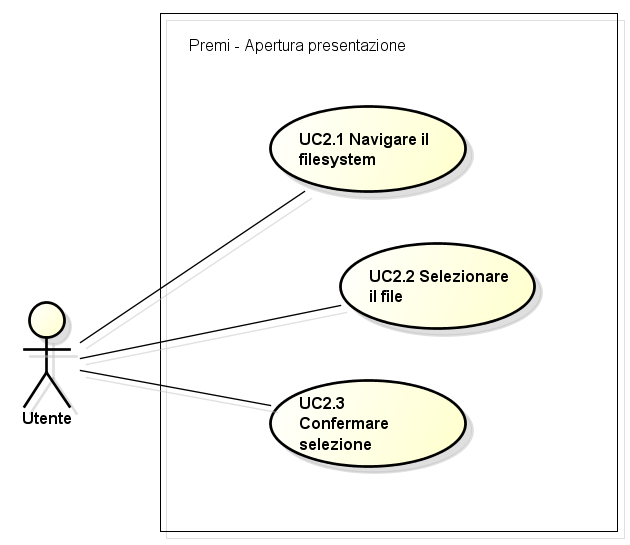
\includegraphics[scale=0.45] {img/UC2.png} 
	\caption{UC2 - Autenticazione} 
\end{figure}

\begin{itemize}
	\item \textbf{Attori:} Proprietario;
	\item \textbf{Scopo e descrizione:} Il proprietario vuole eseguire il login per poter accedere a tutte le sue presentazioni. Compila il modulo di autenticazione, conferma i dati inseriti e, se sono corretti, il sistema gli concede l'accesso;
	\item \textbf{Precondizione:} Il sistema mostra la schermata di login;
	\item \textbf{Flusso degli eventi:}
	\begin{enumerate}
		\item L'utente inserisce le sue credenziali [UC2.1];
		\item L'utente conferma l'inserimento delle credenziali [UC2.2];
		\item Il sistema verifica che le credenziali siano corrette [UC2.3];
		\item Se le credenziali sono errate il sistema lo segnala con un errore [UC2.4];
		\item Le credenziali sono corrette e il sistema permette l'accesso all'utente [UC2.5];
	\end{enumerate}
	\item \textbf{Postcondizione:} Il sistema ha verificato le credenziali e ha consentito l'accesso all'utente.
\end{itemize}

\subsection{Caso d'uso UC2.1: Inserimento credenziali}
\begin{itemize}
	\item \textbf{Attori:} Proprietario;
	\item \textbf{Scopo e descrizione:} Il proprietario inserisce le sue credenziali nel modulo di autenticazione;
	\item \textbf{Precondizione:} Il sistema è in attesa che l'utente inserisca le sue credenziali;
	\item \textbf{Postcondizione:} L'utente ha inserito correttamente i suoi dati.
\end{itemize}

\subsection{Caso d'uso UC2.2: Conferma dati}
\begin{itemize}
	\item \textbf{Attori:} Proprietario;
	\item \textbf{Scopo e descrizione:} Il proprietario deve confermare i dati inseriti precedentemente;
	\item \textbf{Precondizione:} Il sistema è in attesa che l'utente confermi i dati inseriti;
	\item \textbf{Postcondizione:} Il sistema ha accettato la conferma dell'utente.
\end{itemize}

\subsection{Caso d'uso UC2.3: Verifica validità credenziali}
\begin{itemize}
	\item \textbf{Attori:} Proprietario;
	\item \textbf{Scopo e descrizione:} Il sistema verifica la validità dei dati inseriti dal proprietario;
	\item \textbf{Precondizione:} Il sistema ha ricevuto la richiesta di verifica delle credenziali;
	\item \textbf{Postcondizione:} Il sistema ha verificato la correttezza delle credenziali.
\end{itemize}

\subsection{Caso d'uso UC2.4: Errore di autenticazione}
\begin{itemize}
	\item \textbf{Attori:} Proprietario;
	\item \textbf{Scopo e descrizione:} Il sistema segnala all'utente che i dati inseriti non sono corretti e richiede di eseguire nuovamente l'inserimento delle credenziali;
	\item \textbf{Precondizione:} L'utente ha inserito delle credenziali errate;
	\item \textbf{Postcondizione:} Il sistema segnala all'utente che le credenziali inserite sono sbagliate e lo riporta all'inizio della procedura di autenticazione.
\end{itemize}

\subsection{Caso d'uso UC2.5: Accesso al sistema}
\begin{itemize}
	\item \textbf{Attori:} Proprietario;
	\item \textbf{Scopo e descrizione:} Il sistema ha verificato la validità delle credenziali e permette al proprietario l'accesso ai suoi dati;
	\item \textbf{Precondizione:} L'utente ha inserito delle credenziali corrette;
	\item \textbf{Postcondizione:} L'utente ha l'accesso ai suoi dati.
\end{itemize}

\newpage